\documentclass{article}
\usepackage[german]{babel}
\usepackage{graphicx,hyperref,xcolor}

%%%%%%%%%% Start TeXmacs macros
\catcode`\>=\active \def>{
\fontencoding{T1}\selectfont\symbol{62}\fontencoding{\encodingdefault}}
\newcommand{\tminput}[2]{\trivlist{\item[\color{rgb:black,10;red,9;green,4;yellow,2}{#1}]{\color{blue!50!black}\mbox{}#2}}}
\newcommand{\tmoutput}[1]{#1}
\newcommand{\tmsession}[3]{{\tt#3}}
\newcommand{\tmstrong}[1]{\textbf{#1}}
\newcommand{\tmunfoldedio}[3]{\trivlist{\item[\color{rgb:black,10;red,9;green,4;yellow,2}{#1}]\mbox{}{\color{blue!50!black}#2}\item[]\mbox{}#3}}
%%%%%%%%%% End TeXmacs macros

\begin{document}

{\tmstrong{Vorlesung 8 7.06.2016}}

\

\href{/home/christian/Gedankenspeicher/Studium//Comp-NLD-1/Vorl8-A3-11.cpp}{Vorl8-A3-11.cpp}

Numerische L{\"o}sung der Van de Pol Gleichung durch die Methode 'Predictor -
Corrector'

\tmsession{shell}{default}{
  \tmoutput{Shell session inside TeXmacs pid = 13978}
  \tminput{Shell] }{g++ -o Vorl8-A3-11 Vorl8-A3-11.cpp \&\& ./Vorl8-A3-11 >
  V8-A3-11-E1.dat\\
  }
  \tminput{Shell] }{\ }
}

Plot der Van de Pol Gleichung x1 und x2

\tmsession{gnuplot}{default}{
  \tmoutput{This is a TeXmacs interface for GNUplot.}
  \tmunfoldedio{GNUplot] }{plot 'V8-A3-11-E1.dat' using 2:3 \# mu =
  5}{\raisebox{0.0\height}{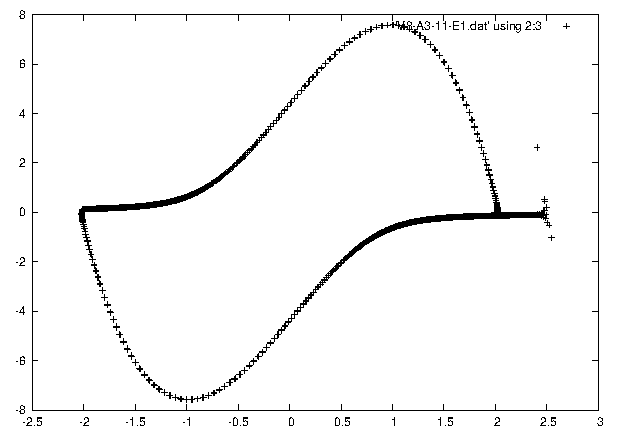
\includegraphics[width=10.411911321002231cm,height=7.288337924701561cm]{Vorlesung-8-1.pdf}}}
  \tminput{GNUplot] }{\ }
}

\

\

\end{document}
